\chapter{Analysis \& Results}
\startcontents[chapters]
\printcontents[chapters]{}{1}{}
\noindent\\
So far the system's design, implementation, and example usage, has been presented and discussed.

\section{Introduction}
This chapter presents analytic information

\section{Implementation Analysis}
This section analysis the synthesised and implemented system-on-chip design to see the effect of increasing core counts.

\subsection{Design Size}
\subsubsection{Constraints}
As discussed in \cref{sec:singlecore} \nameref{sec:singlecore}, each processor core features two memories: instruction and scratch memory, which can both map onto synchronous, single-port, FPGA BRAM blocks. While this will reduce LUT requirements in designs with few cores, it becomes a non-trivial problem as the core counts increase. FPGAs have a fixed number of hard-BRAM blocks available for inference by the HDL compiler, for example the low-end Xilinx Spartan-6 XC6SLX9 FGPA features 32 18 Kb BRAM blocks \cite[p.~2]{s6fam}, and the Cyclone V 5CSEMA5F31C6N (used in the DE1-SoC) has 397 10 Kb blocks \cite[p.~22]{cvfam}.

\begin{figure}[h]
\centering
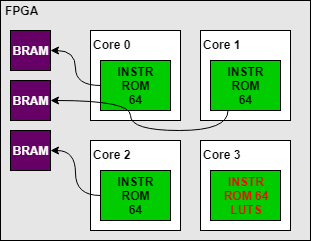
\includegraphics[width=0.5\textwidth]{bram_limit}
\caption{A theoretical FPGA device with 3 BRAM blocks running a 4-core design. Each core can map onto a BRAM block, however as there are more cores than BRAM blocks available, some core memories will be implemented as distributed RAM, or in the worse case using ALMs.}
\label{fig:bram_limit}
\end{figure}

As shown in \cref{fig:bram_limit}, as the number of processor cores increasing they eventually outnumber the available BRAM blocks, resulting in their memories being implemented in either distributed RAMs or ALMs, both of which can consume significant logic resources of the FPGA which reduces the maximum possible core count.

\section{Scenario Performance}
To evaluate the performance of the system-on-chip, scenarios encompassing computational problems that are reflective of real-world applications are compiled and ran on the design.

\subsection{Scenario Overview}
The scenario is a software program that runs a parallel implementation of the summation function, i.e. \verb|sum [1..10]| which returns 55. While this may seem too simple at first to measure performance of a multi-core system-on-chip, the function is actually quite appropriate as it encompasses various parallel problems, such as: a fixed time/size serial part; broadcasting of the data set (in this case the range of the summation); thread synchronisation (to know when the data is ready and to schedule gathering of intermediary results); and is highly scalable.
\\\\
The summation task flow is as follows:
\begin{enumerate}
\item Root (core \#0) broadcasts the range of the summation (i.e. sum 1 to 10) to all cores via the global shared memory.
\item Non-root cores wait for this broadcast to finish (memory barrier), then calculate their own subset of the range to sum. For example, if Root broadcasts that there are 240 samples and 10 cores in the system, each core calculates the subset size:

\begin{equation}
240/10 = 24
\end{equation} calculations starting from:
\begin{equation}
{ID_{CORE}} * 24
\end{equation}
For example, Core \#5 will start its 24 sample subset summation from
\begin{equation}
5 * 24 = 120
\end{equation}
effectively performing \verb|sum [120..123]|.

\item All cores perform an intermediary summation over their subset of the range (serial part).
\item All cores attempt to add their intermediary result to a global sum value in global shared memory (mutex).
\item All cores halt, signalling that their work has been committed to the global shared memory and have finished the program.
\end{enumerate}

This program is written in assembly in the file \verb|sw/demos/asm/sum64.s| and can be compiled using the assembly compiler (developed for deliverable \ref{ed:compiler}) using the command below. The assembly compiler outputs the file \verb|asm.s.hex| containing hex instruction words for use in Verilog's \verb|$readmemh| function. This data is used for each core's instruction memory. The assembly program is also shown in \cref{sec:64coresum}.
\\
\mintinline{bash}{                      python sw/asm.py sw/demos/asm/sum64.s}

\subsection{Performance Measurements}
Behavioural simulation will be used to measure the following metrics to estimate general performance of the system-on-chip:
\begin{itemize}
\item Total program run-time.\\This is the time from when the reset signal is de-asserted to when all cores have halted. Each core has an output \verb|halt| signal which the SoC can use to determine if all cores have halted using \verb|wire all_halted = &core_halts;|. 

\item Time spent on the serial part.\\The serial part of this scenario consists of the intermediary summation of it's subset range. As each core is performing this task, the average will be used.

\item Time spent on communication.\\This includes time spent on thread synchronisation, i.e. waiting for the global memory to become available and waiting on the root to finish broadcast. Again, the average time will be used.

\item Time spent fetching instructions.\\Instruction fetches occur during stage \verb|STAGE_IF| of the pipeline. The behavioural test bench will record the number of clock cycles each core spends in this state, then calculate the average time spent fetching instructions. 
\end{itemize}

\subsection{Performance Results}
\begin{figure}[h]
\centering
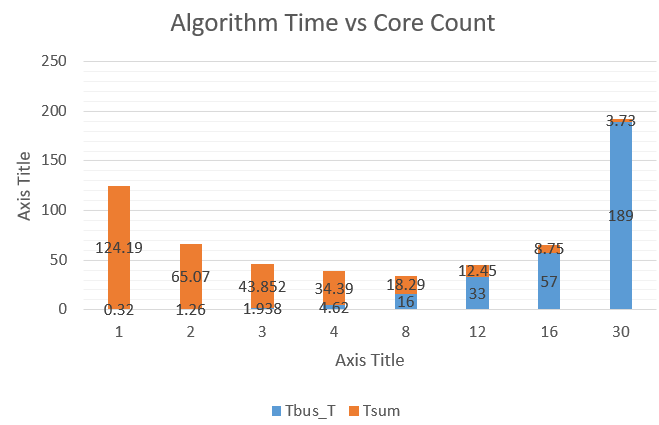
\includegraphics[width=0.7\textwidth]{alg_time}
\caption{Chart showing how the communication times (Tbus) and serial times (Tsum) changes with core count.}
\label{fig:alg_time}
\end{figure}

\begin{figure}[h]
\centering
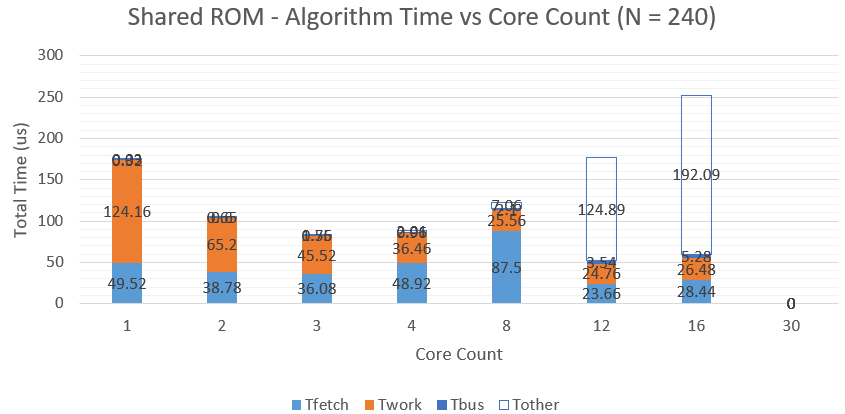
\includegraphics[width=0.7\textwidth]{alg_time_shared}
\caption{Similar to \cref{fig:alg_time} but using shared instruction memory to reduce block memory requirements per core.}
\label{fig:alg_time_shared}
\end{figure}















